\documentclass[crop,tikz]{standalone}
\usetikzlibrary{backgrounds}
\colorlet{blue}{cyan}
\tikzset{
  inverted/.style = {
    color=white,
    background rectangle/.style={fill},
    show background rectangle
  }
}

\usepackage[european]{circuitikz}

\begin{document}
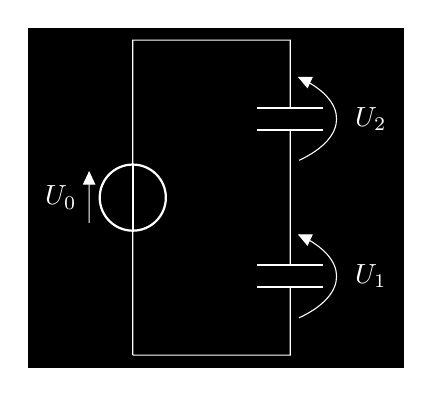
\begin{tikzpicture}[inverted,inverted]
  \draw (0,-2)
    to[V,v=$U_0$] ++(0,4)
    to[short] ++(2,0)
    to[C,v^<=$U_2$] ++(0,-2)
    to[C,v^<=$U_1$] ++(0,-2)
    to[short] ++(-2,0);
\end{tikzpicture}
\end{document}
